%!TEX root = ../hycas2010.tex
%%%%%%%%%%%%%%%%%%%%%%%%%%%%%%%%%%%%%%%%%%%%%%%%%%%%
\section{The BDI Learning Framework}\label{sec:framework}
%%%%%%%%%%%%%%%%%%%%%%%%%%%%%%%%%%%%%%%%%%%%%%%%%%%%

Our learning task may be summarised as follows: \textit{Given past execution data and the current world state, determine which plan to execute next in order to best address the event-goal in question}. In the BDI sense, our task is to learn the context condition of each plan in the goal-plan hierarchy. In this section we describe our BDI Learning Framework that enables such learning. In particular we describe the use of \dt s for learning context conditions and the confidence-based probabilistic plan selection that incorporates this learning, while focusing on parameterised event-goals and recursion.

%%%%%%%%%%%%%%%%%%%%%%%%%%%%%%%%%%%%%%%%%%
\subsection{Integrating Decision Trees into Context Conditions for Plans}
\label{sec:decision_trees}
%%%%%%%%%%%%%%%%%%%%%%%%%%%%%%%%%%%%%%%%%%

A plans context condition is a logical formula that is constructed at design time and evaluated against an event-goal at run time to determine if the plan is applicable in the given world state\footnote{Context formulas may reference internal beliefs as well as environment states, and for this study we treat both as included in the world state.}. To allow the context condition to be learnt over time, we annotate each plan's context formula with a \textit{\dt}\footnote{It is perfectly feasible to combine the existing logical formula with the \dt\ classification, but to aid our understanding of the \dt\ learning in this study we always use an empty initial formula.}\cite{Airiau:IJAT:09}. The idea is that the agent starts with some \textit{necessary but possibly insufficient} conditions for each plan (provided by the designer), and over time and in the course of trying plans in various world states will \textit{refine} each plan's context condition using the learnt \dt.
 
The choice of \dt s for learning is motivated by several factors. Firstly, \dt s support hypotheses that are a disjunction of conjunctive terms and this representation is compatible with how context formulas are generally written. Secondly, \dt s can be converted to \textit{if-then} rules that are human readable and can be validated by a domain expert. Finally, \dt s are robust against training data that may contain errors. This is specially relevant in stochastic domains where applicable plans may nevertheless fail due to unforeseen circumstances.

For each plan, the training set for its \dt\ contains samples of the form $[w,o]$, where $w$ is the world state in which the plan was executed and $o$ was the boolean outcome (success or failure). The world state $w$ itself is a set of discrete attributes that together represent the state of affairs. Initially the training set is empty and grows as the agent tries the plan in various world states and records each result. Over time the \dt\ learnt from the training set will contain only those attributes of world state $w$ that are relevant to that plans context condition.

The number of attributes in world state $w$ and their range has a bearing on the size of the training set required to correctly learn the context condition. In general, world state $w$ should be constructed with all attributes that are possibly relevant to the context condition. For instance, for a plan to pick objects using a robotic arm, the attributes \textit{objectSurface} and \textit{gripperWet} are likely relevant and should be included, while the attribute \textit{dayOfWeek} possibly is not and may be exluded. The choice of attributes to include in the world state $w$ is eventually a design decision and dependent on domain knowledge. For our purposes we assume that the designer provides a set of all attributes that are considered \textit{possibly relevant} to the context condition of the plan. In the worst case, this set is the full set of available attributes. 

The decision tree inductive bias is a preference for smaller trees. In other words, the induction of \dt s will trade-off some accuracy in classification for compactness of representation. In fact such inductive bias is necessary if the \dt\ is to generalise to as yet unseen world states. Once a \dt\ is induced from the training set, it may be used to classify any new world state $w$. In the strict sense the classification is an outcome $o$ (failure or success). However, several \dt\ implementations including \propername{J48} in \weka\footnote{In our study we use algorithm \propername{J48}, a version of \propername{c4.5} \cite{Mitchell97:ML}, from the \weka\ learning package \cite{weka99}.} annotate a likelihood of class membership (that is indicative of the inductive bias) to the returned classification. For the given world state $w$ then, we treat the returned likelihood of membership to the $success$ class as the expected likelihood of success of the plan.


%%%%%%%%%%%%%%%%%%%%%%%%%%%%%%%%%%%%%%%%%%
\subsection{Support for Recursive Event-Goals}
%%%%%%%%%%%%%%%%%%%%%%%%%%%%%%%%%%%%%%%%%%

Recursion in our context refers to the case where the resolution of an event-goal instance $G(\vec{x_1})$ involves first the resolution of goal-event instance $G(\vec{x_2})$ of the same type $G$. The result is a growing stack of pending $G(\vec{x_i})$ event-goals that eventually terminate in $G(\vec{x_n})$ whose parameters satisfy the termination conditions where a non-recursive plan choice is made.

In order to understand the impact of recursion on context learning, we use the notion of an \textit{execution trace} of the form $G_0(\vec{x_0})[P_0:w_0] \cdot G_1(\vec{x_1})[P_1:w_1] \cdot \ldots \cdot G_n(\vec{x_1})[P_n:w_n]$, that represents a sequence of event-goals along with the plans selected to handle them and the world state in which the selections were made. So $G_i(\vec{x_i})[P_i:w_i]$ captures the case where plan $P_i$ was selected in world state $w_i$ in order to achieve the goal-event $G_i(\vec{x_i})$.

\begin{figure}[t]
\begin{center}
\resizebox{0.8\textwidth}{!}{
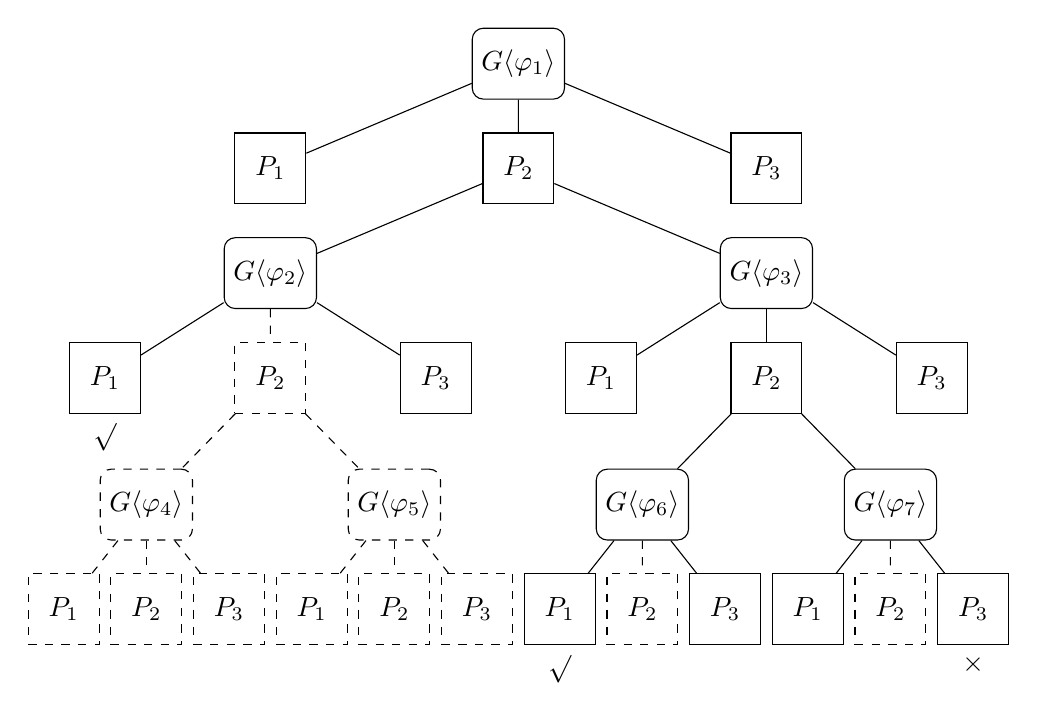
\begin{tikzpicture}[scale=0.7]
\tikzstyle{txt}=[scale=1.0]
\tikzstyle{succ}=[label=below:$\surd$]
\tikzstyle{fail}=[label=below:$\times$]
\tikzstyle{planbox}=[draw,minimum height=0.9cm,minimum width=0.9cm]
\tikzstyle{goalbox}=[draw,rounded corners,minimum height=0.9cm,minimum width=1.0cm]
\tikzstyle{level 1}=[sibling distance=4.5cm,level distance=1.9cm] 
\tikzstyle{level 2}=[sibling distance=9.0cm,level distance=1.9cm] 
\tikzstyle{level 3}=[sibling distance=3.0cm,level distance=1.9cm]
\tikzstyle{level 4}=[sibling distance=4.5cm,level distance=2.3cm]
\tikzstyle{level 5}=[sibling distance=1.5cm,level distance=1.9cm]
\tikzstyle{level 6}=[sibling distance=1.3cm,level distance=1.9cm]

\node[goalbox,yshift=1cm] {$G\langle\varphi_1\rangle$}
	child {node[planbox] {$P_1$}}
	child {node[planbox] {$P_2$}
		child {node[goalbox] {$G\langle\varphi_2\rangle$}
			child {node[planbox,succ] {$P_1$}}
			child[dashed] {node[planbox] {$P_2$}
				child {node[goalbox] {$G\langle\varphi_4\rangle$}
					child {node[planbox] {$P_1$}}
					child {node[planbox] {$P_2$}}
					child {node[planbox] {$P_3$}}
				}
				child {node[goalbox] {$G\langle\varphi_5\rangle$}
					child {node[planbox] {$P_1$}}
					child {node[planbox] {$P_2$}}
					child {node[planbox] {$P_3$}}
				}
			}
			child {node[planbox] {$P_3$}}
		}
		child {node[goalbox] {$G\langle\varphi_3\rangle$}
			child {node[planbox] {$P_1$}}
			child {node[planbox] {$P_2$}
				child {node[goalbox] {$G\langle\varphi_6\rangle$}
					child {node[planbox,succ] {$P_1$}}
					child[dashed] {node[planbox] {$P_2$}}
					child {node[planbox] {$P_3$}}
				}
				child {node[goalbox] {$G\langle\varphi_7\rangle$}
					child {node[planbox] {$P_1$}}
					child[dashed] {node[planbox] {$P_2$}}
					child {node[planbox,fail] {$P_3$}}
				}
			}
			child {node[planbox] {$P_3$}}
		}
	}
	child {node[planbox] {$P_3$}}
;

\end{tikzpicture}

}
\end{center}
\caption{Goal-plan hierarchy containing a parameterised goal $G$ handled by three plans $P_1$, $P_2$ and $P_3$. Here plan $P_2$ posts two instances of $G$ resulting in recursion. Two levels of recursive unfolding are shown. Dashed $P_2$ nodes indicate unexplored recursive sub-trees.}
\label{fig:unfolding}
\end{figure}

Consider the example BDI goal-plan hierarchy of Figure \ref{fig:unfolding}. The structure has just a single parameterised goal $G$ and three options to handle it, one of which, $P_2$, in turn posts two instances of the same parameterised goal $G$. In this way, the only plans that take an action in the environment are $P_1$ and $P_3$. The figure highlights an execution trace as follows: \[
\lambda=G(\vec{x_1})[P_2:w_1] \cdot G(\vec{x_2})[P_1:w_1] \cdot G(\vec{x_3})[P_2:w_2] \cdot G(\vec{x_6})[P_1:w_2] \cdot G(\vec{x_7})[P_3:w_3].
\]

The first choice in the execution results in the selection of plan $P_2$ to handle event-goal instance $G(\vec{x_1})$ in a given world $w_1$. Plan $P_2$ in turn immediately posts the event-goal instance $G(\vec{x_2})$ that is successfully handled by the non-recursive node $P_1$. Plan $P_2$ then posts the second event-goal instance $G(\vec{x_3})$, which then is handled by itself in a recursive manner.  The outcome is that $\lambda$ traces a path that involves the successive execution of leaf plan $P_1$ for event-goal $G(\vec{x_2})$ followed by another execution of $P_1$ for event-goal $G(\vec{x_6})$, finally terminating in the failure of leaf plan $P_3$ for event-goal $G(\vec{x_7})$. Note that if plan $P_2$ had instead been selected to handle $G(\vec{x_7})$ then a deeper recursive call would have ensued. Similarly if earlier in the execution trace plan $P_2$ was selected to handle event-goal $G(\vec{x_2})$ then a different recursive sub-tree (shown in Figure \ref{fig:unfolding} as dotted nodes under $G(\vec{x_2})$) would have unfolded.

The immediate implication of a recursive goal-plan structure is that the size of the hierarchy is no longer static but instead unfolds in a dynamic manner. The risk then is that since the conditions that terminate recursion are not ready at the start (we are trying to learn them), then the agent may get trapped in an infinite recursive loop during exploration. This has implications for any strategy that relies on the structure being finite. For instance, our conservative recording approach \cite{Airiau:IJAT:09} and coverage-based confidence measure \cite{Singh:AAMAS10} both suffer from this problem. Incidentally, the simpler aggressive recording approach \cite{Airiau:IJAT:09} is not impacted by recursion as it does not consider the goal-plan structure.

One way to resolve this issue is to treat all recursive goals simply as sub-trees in a static structure and limit the recursive \textit{unfolding}  to a maximum allowed depth. In this study we use this bounded recursion approach for handling recursive structures. It follows then that wherever a recursive structure applies, a maximum recursion value must be supplied. This may not be an unrealistic requirement given that the domain expert will usually have some idea of how much recursion is sufficient for a given parameterised event-goal. 

%%%%%%%%%%%%%%%%%%%%%%%%%%%%%%%%%%%%%%%%%%
\subsection{Calculating Confidence in the Decision Tree Classification}
%%%%%%%%%%%%%%%%%%%%%%%%%%%%%%%%%%%%%%%%%%

The typical use of \dt s lies in the \textit{offline} induction from a complete training set. In that sense, the use of \dt s in our framework is unorthodox since the training set is built incrementally by recording samples after each new execution. This results in the training set being incomplete\footnote{Training data is incomplete in the sense that the agent has only collected a portion of the full data set required to learn the correct classification.} in the early stages of learning leading to misclassification. A confidence measure in the \dt\ classification is therefore desirable to address this issue. Previously \cite{Singh:AAMAS10} we showed how the coverage of possible execution paths below the plan in the goal-plan hierarchy may be used to build such a measure. Here we propose a new confidence measure that builds on the idea but that does not suffer from its limitations (Section \ref{subsec:bdi_learning}).

Our requirement for the confidence measure is that it be a monotonic function whose values transition from no confidence ($0.0$) to full confidence ($1.0$) based on experience. Specifically, the experiences we are interested in should constitute coverage of the plan complexity (number of sub-plan choices) and the domain complexity (number of world states in which the plan applies). Since an exact calculation of such coverage does not scale for all practical purposes then we are interested in an \textit{approximate} coverage that is still representative of the state of affairs but is simpler to compute.

One way to achieve this is to use a monotonic decay function\footnote{This technique is frequently applied in machine learning algorithms for balancing between exploration of choices and exploitation of learning.} (for instance $\epsilon_i = \epsilon_{i-i} * \delta$ where $\delta < 1.0$) but where the decay factor $\delta$ is tied to the complexity involved. This way, a plan that has a larger number of sub-plan choices will utilise a slower decay factor $\delta$ taking longer to reach full confidence $(1-\epsilon)$ than another plan that has less choices to make. For goal-plan complexity this decay $\delta_{Pt}$ may be calculated offline by analysing the goal-plan hierarchy. In this work, we have calculated $\delta_{Pt}$ in terms of average breadth and depth of the structure, where depth is the maximum level of recursion in this case, to provide an approximation of the complexity of the structure\footnote{There are other ways of calculating $\delta_{Pt}$ (e.g., in \cite{Singh:AAMAS10} we have used an accurate calculation of the number of choices below plans; however this is not feasible anymore when goals and plans are schemas with possibly infinite instances); the main idea is to somehow measure the complexity of a hierarchical structure, and is the subject of ongoing work.}. A similar treatment is possible for domain complexity although the decay factor in this case cannot be pre-determined since the number of world states is not known upfront and is dependent on the domain. For domain complexity then, it may be reasonable to treat the decay factor $\delta_{Pd}$ as a parameter specified by the domain expert.

\begin{equation}\label{eqn:confidence}   
c_P = (1.0 - \epsilon_{Pt}) * (1.0 - \epsilon_{Pd}).
\end{equation}

Equation \ref{eqn:confidence} shows how the final confidence $c_P$ is calculated for a given plan $P$. Here $\epsilon_{Pt}$ is the plans tree complexity decay while $\epsilon_{Pd}$ is the plans domain complexity decay. The actual updates to the decay values are performed each time the plan $P$ is executed while the rate of decay is governed by the decay factors $\delta_{Pt}$ and $\delta_{Pd}$ accordingly.


%%%%%%%%%%%%%%%%%%%%%%%%%%%%%%%%%%%%%%%%%%
\subsection{Handling Parameterised Event-Goals}
%%%%%%%%%%%%%%%%%%%%%%%%%%%%%%%%%%%%%%%%%%

Our BDI learning framework account presented earlier \cite{Airiau:IJAT:09,Singh:AAMAS10} did not account for \textit{parameterised event-goals} but only for event-goal instances. In practical BDI systems, it is often the case that a single plan will handle all instances of a parameterised event-goal. Furthermore event-goal instance parameters will generally be included in the context logical formula. 

Consider again the goal-plan structure in Figure \ref{fig:unfolding} and the highlighted solution path terminating in the leaf plans indicated by the $\surd$ symbol. An important point here is that the indicated solution applies to the event-goal \textit{instance} $G(\vec{x_1})$ and to that instance alone. For a different instance $G(\vec{y_1})$ the solution path would likely be different (one way to visualise this in the Figure \ref{fig:unfolding} is to think of it as an animation where the event-goal parameters and the placement of the $\surd$ symbols changes on each frame).  This means that event-goal instance parameters must also be considered as input for a plan's \dt\ in order to learn solutions per event-goal instance.

We include such an account by augmenting the training samples for the \dt\ with the event-goal parameters. As such, the training set now contains samples of the form $[w,x,o]$ where the world state $w$ is the initial set of all relevant attributes that represent the state of affairs, $x$ is the set of all event-goal parameters, and $o$ is the outcome class (success or failure). Incorporating the event-goal parameter set $x$ in the training data is sufficient for learning with parameterised event-goals, and no fundamental change to the framework is required.

%%%%%%%%%%%%%%%%%%%%%%%%%%%%%%%%%%%%%%%%%%
\subsection{Calculating Plan Selection Weights based on Confidence}
%%%%%%%%%%%%%%%%%%%%%%%%%%%%%%%%%%%%%%%%%%


Typical BDI platforms offer several mechanisms for plan selection from a set of applicable plans, such as plan precedence and meta-level reasoning. However, since these mechanisms are pre-programmed and do not take into account the experience of the agent, we provide a new \textit{probabilistic plan selection} function for this purpose. 

For each plan, given its expectation of success (as determined by its \dt\ learning) and a confidence measure in this expectation (based on coverage), we calculate a final \textit{selection weight} that is indicative of the likelihood of the plan being selected for execution. Equation \ref{eqn:weight} shows how the plan selection weight $\Omega_P(w)$ is calculated for a given world state $w$. Initially, the confidence $c_P$ is zero and the weight takes the default value of $0.5$. Over time, as the confidence improves towards the final value of $1.0$, the selection weight approaches the value $\kappa_P(w)$ estimated by the plan's \dt.


\begin{equation}\label{eqn:weight}   
\Omega_P(w) = 0.5 + \left[  c_P *  \left( \kappa_P(w) - 0.5 \right)  \right].
\end{equation}


Given the set of applicable plans for resolving event-goal $G$ in world state $w$ then, our probabilistic plan selection mechanism chooses a plan $P_i$ with a probability directly proportional to its selection weight $\Omega_{P_i}(w)$. Such selection ensures a balance between the \emph{exploitation} of current know-how and the \textit{exploration} of new choices that is necessary for online learning tasks. 


%Simplifications: Only single level goal recursion allowed ie G1->P1->G1 and not  G1->P1->G2->P2->G. Also no information of Gs in the system so only the parent goal recursion is tracked.

